\documentclass[conference]{IEEEtran}
 
\usepackage{cmap}
\usepackage[T1]{fontenc}


\usepackage{graphicx,url}
\usepackage[table,xcdraw]{xcolor}

\usepackage{times}
\usepackage{latexsym}
 \usepackage[printonlyused]{acronym}
 
\usepackage{blindtext}
\usepackage{graphicx}
\usepackage{amsmath}
\usepackage{kpfonts}
\usepackage{url}
\usepackage{listings}
\usepackage{multirow}
\usepackage{booktabs} 
\usepackage{pgfplots}
\usepackage{graphicx}
\usepackage{cancel}
\usetikzlibrary{patterns}
\pgfplotsset{width=10cm,compat=1.9}


\usepackage{color}

\usepackage{url}

\usepackage{amsmath}
\usepackage{amssymb}


\acrodef{pots}[POTS]{Poverty of the Stimulus}

\acrodef{CBIR}{Content-based image retrieval}
\acrodef{MAM}{Metric Access Method}
\acrodef{AM}{Access Method}
\acrodef{SAM}{Spatial Access Method}
\acrodef{MST} {Minimum Spanning Tree}
\acrodef{IR} {Information Retrieval}
\acrodef{NDC} {Number of Distance Calculations}
\acrodef{LAESA} {Linear Approximating Eliminating Search Algorithm}
\acrodef{AESA} {Approximating Eliminating Search Algorithm}
\acrodef{RNG} {Relative Neighborhood Graph}
\acrodef{DT} {Delaunay Triangulation}
\acrodef{GG} {Gabriel Graph}
\acrodef{UG} {Urquhart Graph}
\acrodef{SAT} {Spacial Approximation Tree}
\acrodef{RNDF} {Relative Neighborhood Density Factor}
\acrodef{NN} {Nearest Neighbor}
\acrodef{NAG} {Neighborhood Approximation Graph}
\acrodef{HRG} {Hyperspherical Region Graph}
\acrodef{NA-Graph} {Neighborhood Approximation Graph}
\acrodef{DA} {Disk Access}
\acrodef{DTW} {Dynamic Time Warping}
\acrodef{LSH} {Locality Sensitive Hashing}
\acrodef{CNN} {Convolutional Neural Network}
\acrodef{CNNs} {Convolutional Neural Networks}

\usepackage{pgfplotstable,booktabs}
%%%%%%%%%%%%%%%%%%%%%%%%%%%%%%%%%%%%%%%%%%%%%%
%% You don't need this part
% I did it to create your file 
\usepackage{filecontents} % <-- To create files on the fly


% Needed packages
\usepackage{tikz}
\usepackage{pgfplots}
\pgfplotsset{compat=newest}

% Command to read a number from file (the hspace is quite hacky...)
\newcommand{\showodsf}[2]{%
\mbox{\input{data/#1_#2_ods_f.txt}\hspace{-2.5pt}}%
}

\newcommand{ \Correction }[ 1 ] {\textcolor{black}{#1}}
\newcommand{ \NewMaterial }[ 1 ] {\textcolor{black}{#1}}
\newcommand{ \ConnectDots }[ 1 ] {\textcolor{black}{#1}}
 
%english has to go last to set it as default language
\usepackage[ngerman,english]{babel}
%Hint by http://tex.stackexchange.com/a/321066/9075 -> enable "= as dashes
\addto\extrasenglish{\languageshorthands{ngerman}\useshorthands{"}}

%better font, similar to the default springer font
%cfr-lm is preferred over lmodern. Reasoning at http://tex.stackexchange.com/a/247543/9075
\usepackage[%
rm={oldstyle=false,proportional=true},%
sf={oldstyle=false,proportional=true},%
tt={oldstyle=false,proportional=true,variable=true},%
qt=false%
]{cfr-lm}
 
%for easy quotations: \enquote{text}
\usepackage{csquotes}

%enable margin kerning
\usepackage{microtype}

%tweak \url{...}
\usepackage{url}
%\urlstyle{same}
%improve wrapping of URLs - hint by http://tex.stackexchange.com/a/10419/9075
\makeatletter
\g@addto@macro{\UrlBreaks}{\UrlOrds}
\makeatother
%nicer // - solution by http://tex.stackexchange.com/a/98470/9075
%DO NOT ACTIVATE -> prevents line breaks
%\makeatletter
%\def\Url@twoslashes{\mathchar`\/\@ifnextchar/{\kern-.2em}{}}
%\g@addto@macro\UrlSpecials{\do\/{\Url@twoslashes}}
%\makeatother

%diagonal lines in a table - http://tex.stackexchange.com/questions/17745/diagonal-lines-in-table-cell
%slashbox is not available in texlive (due to licensing) and also gives bad results. This, we use diagbox
%\usepackage{diagbox}

%required for pdfcomment later
\usepackage{xcolor}


%enable nice comments
%this also loads hyperref
\usepackage{pdfcomment}
%enable hyperref without colors and without bookmarks
\hypersetup{hidelinks,
   colorlinks=true,
   allcolors=black,
   pdfstartview=Fit,
   breaklinks=true}
%enables correct jumping to figures when referencing
\usepackage[all]{hypcap}

\newcommand{\commentontext}[2]{\colorbox{yellow!60}{#1}\pdfcomment[color={0.234 0.867 0.211},hoffset=-6pt,voffset=10pt,opacity=0.5]{#2}}
\newcommand{\commentatside}[1]{\pdfcomment[color={0.045 0.278 0.643},icon=Note]{#1}}

%compatibality with packages todo, easy-todo, todonotes
\newcommand{\todo}[1]{\commentatside{#1}}
%compatiblity with package fixmetodonotes
\newcommand{\TODO}[1]{\commentatside{#1}}

%enable \cref{...} and \Cref{...} instead of \ref: Type of reference included in the link
\usepackage[capitalise,nameinlink]{cleveref}
%Nice formats for \cref
\crefname{section}{Sect.}{Sect.}
\Crefname{section}{Section}{Sections}

\usepackage{xspace}
%\newcommand{\eg}{e.\,g.\xspace}
%\newcommand{\ie}{i.\,e.\xspace}
\newcommand{\eg}{e.\,g.,\ }
\newcommand{\ie}{i.\,e.,\ } 
  
\begin{document}
% 
% Do not put math or special symbols in the title.
\title{Approximate nearest neighbors by  deep learning hashing on large-scale search}



% author names and affiliations
% use a multiple column layout for up to three different
% affiliations
\author{\IEEEauthorblockN{Michael Shell}
\IEEEauthorblockA{School of Electrical and\\Computer Engineering\\
Georgia Institute of Technology\\
Atlanta, Georgia 30332--0250\\
Email: http://www.michaelshell.org/contact.html}
\and
\IEEEauthorblockN{James Kirk\\ and Montgomery Scott}
\IEEEauthorblockA{Starfleet Academy\\
San Francisco, California 96678--2391\\
Telephone: (800) 555--1212\\
Fax: (888) 555--1212}} 

% make the title area
\maketitle

% As a general rule, do not put math, special symbols or citations
% in the abstract
\begin{abstract}

An optimal data representation  is  an important  task in information retrieval.   A fast indexing method increases the performance level and a good representation offers precise discrimination.  

%In this work we perform exhaustive experiments  
        
Hashing produces  compact representation for  data, to perform task like classification or retrieval based on these short codes. 

When hashing is supervised, the codes are trained using labels on the training data.

Evaluation protocols used in the literature for supervised hashing are not satisfactory. 

We show that a trivial solution that encodes the output of a classifier significantly outperforms existing supervised or semi-supervised methods, while using much shorter codes. 

We propose two alternative protocols for supervised hashing: one based on retrieval on disjoint set of classes, and another based on transfer learning to new classes. We provide two baseline methods for image-related tasks to assess the performance of semi-supervised hashing: without coding and with unsupervised codes. 

These baselines give a lower- and upper-bound on the performance of a supervised hashing scheme. 
%%%%%%%%%%%%%%%%%%%%

Evalution using the class-wise splitting protocol:

To further evaluate our hashing method based on class-wise labels as nearest neighbor, we followed an alternative evaluation protocol [56] which uses disjoint set of classes for training and testing. This is to show that our method is still effective in preserving the ssemantic information of certain classes implicitly even if these class samples are not included in the training set. Specifically, we separated the samples based on class splits such that we used 70% of the classes for training, and 30% of the classes for testing. 

The samples that belong to the 30% of fthe classes was then separated into gallery and query set similar to the previous experiment. 
  
%####################
Both image-text and text-image retrieval modes are considered. Traditionally, class labels in the training and testing sets are identical. That is, it is usually assumed that the query falls into some pre-defined classes. 

However, in practice, the content of a query image/text may vary extensively, and the retrieval system does not necessarily know in advance the class label of a query. Considering the inconsistency between the real world applications and laboratory assumptions, we think that the existing protocol that works under identical train/test classes can be modified and improved.
 


%%%%%%%%
In this Similarity search algorithms based on hashing were proposed to query high-dimensional datasets due to its fast retrieval speed and low storage cost.   Recent studies, promote the use of  \ac{CNN} with hashing techniques to improve the search accuracy.  However, there are challenges to solve in order to find a practical and efficient solution to index CNN features, such as the need for heavy training process to achieve accurate query results and the critical dependency on data-parameters.   Aiming to overcome these issues, we propose a new method for scalable similarity search, i.e., Deep frActal based  Hashing (DAsH), by computing the best data-parameters values for optimal sub-space projection  exploring the correlations among CNN features attributes using fractal theory. Moreover, inspired by recent advances in CNNs, we use not only activations of lower layers which are more general-purpose but also previous knowledge of the semantic data on the latest CNN layer to improve the search accuracy.  Thus, our method produces a better representation of the data space with a less computational cost for a better accuracy.  This significant gain in speed and accuracy allows us to evaluate the framework on a  large, realistic, and challenging set of datasets.  

\end{abstract}

% no keywords

 
\IEEEpeerreviewmaketitle


 
\section{SUPERVISED HASHING}
Compress a set of vectors and their labels  $((x_i,y_2))^{n}_{i=1}, x_1\in R^{d}, y_1 \in \{1,...,L\} $


 
\begin{figure}[htp]
 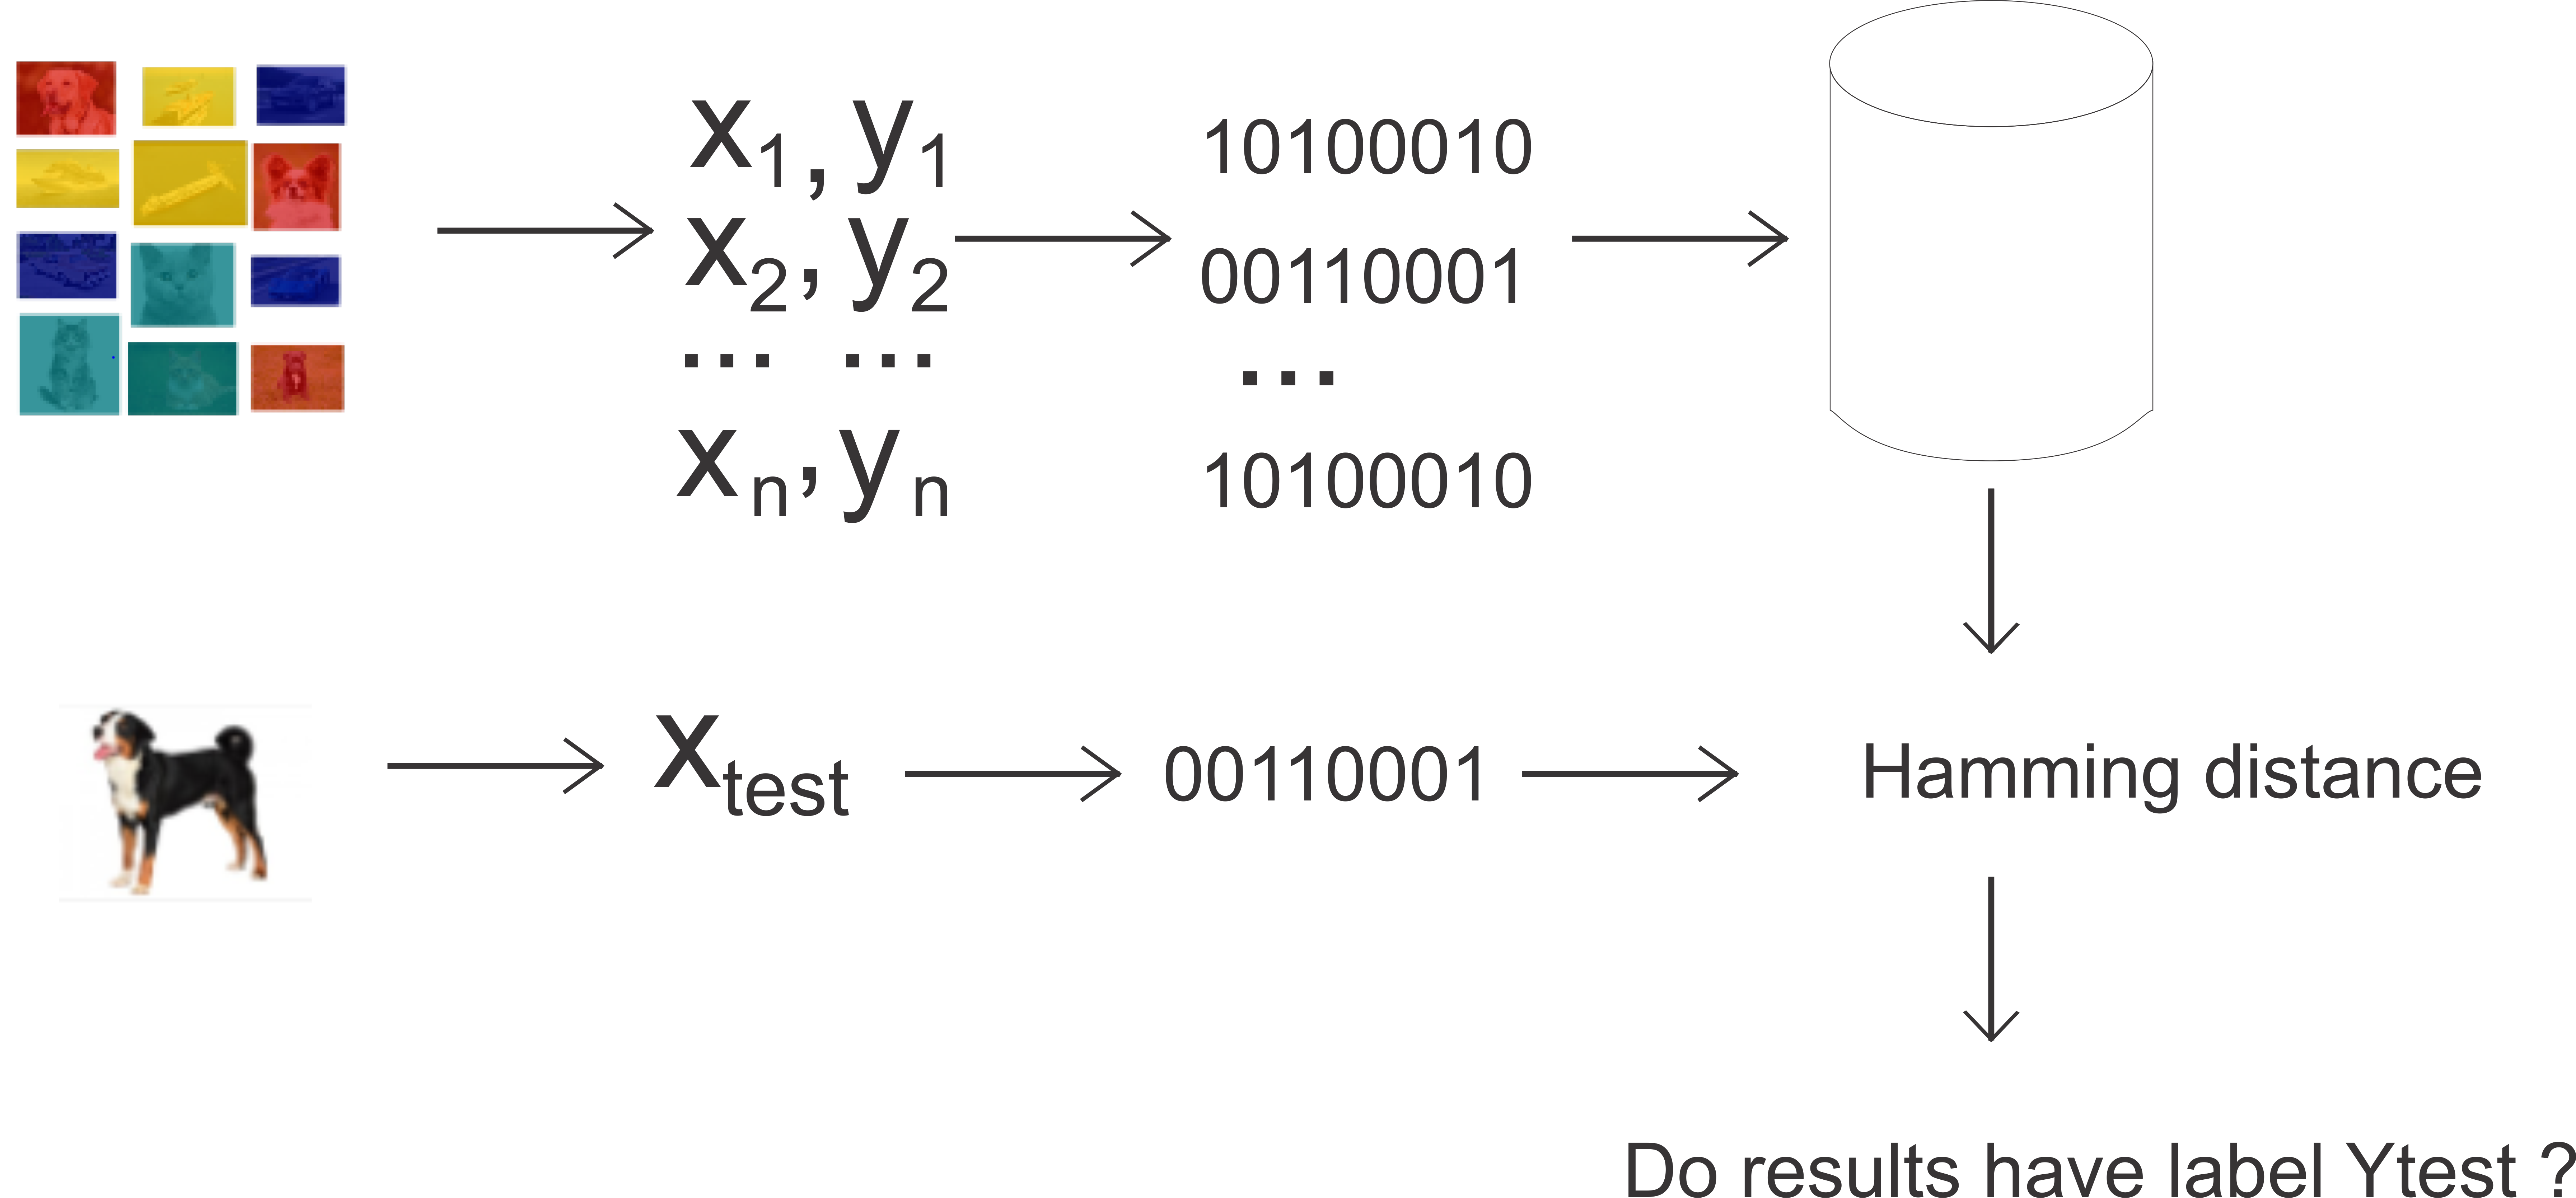
\includegraphics[width=8cm]{dash/12.png} 
 \centering

\caption{ HASHING FOR NEAREST NEIGHBOR SEARCH } 
\end{figure}

\begin{itemize}
\item Supervised hashing $[1, 2]$: labels $y$ known for all $x$ in the reference set
\item Semi-supervised hashing $[3, 4]$: labels $y$ known for only $n_label$ samples

\end{itemize}
 
\subsection{HOW CAN WE AVOID THIS BIASED PROTOCOL?}

\ref{fig:13}.  
\begin{figure*}[htp]\centering
\label{fig:13}
 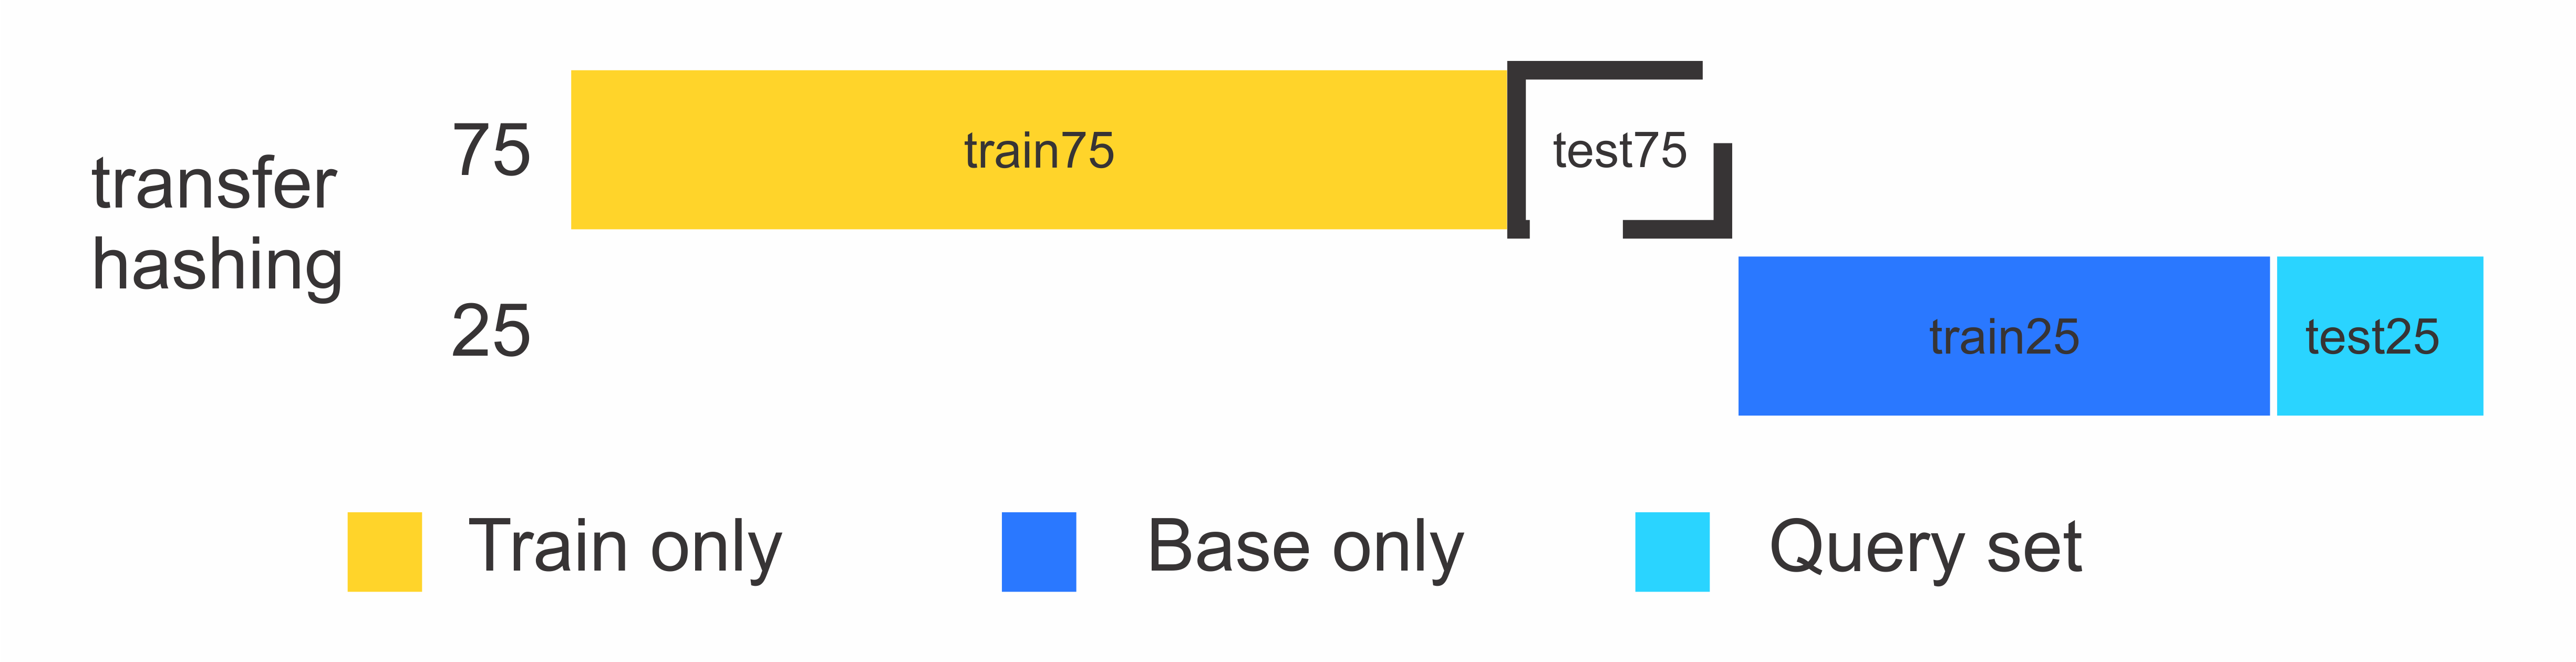
\includegraphics[width=8cm]{dash/13.png} 

\end{figure*}


 

% that's all folks
\end{document}


